\documentclass{article}
\usepackage[T1]{fontenc}
\usepackage{lmodern}
\usepackage{graphicx}
\usepackage{amsmath,amssymb}
\usepackage[a4paper,margin=2cm]{geometry}
\usepackage[absolute,overlay]{textpos}
\setlength{\TPHorizModule}{1mm}
\setlength{\TPVertModule}{1mm}
\usepackage[indonesian]{babel}
\usepackage{hyperref}
\setlength{\emergencystretch}{2em}
% unit: Halaman 5

\begin{document}

% === Halaman 5 (llm) ===

% (tidak ada teks dari model)

% deskripsi: Diagram hierarki Kriptologi yang terbagi menjadi Kriptografi dan Kriptanalisis, dengan rincian lebih lanjut untuk Kriptografi menjadi Klasik (Substitusi, Transposisi) dan Modern (Simetrik, Asimetrik), serta Kriptanalisis menjadi Klasik dan Modern.
% bbox normalisasi: [0.0680, 0.2020, 0.9270, 0.7210]
\begin{textblock*}{180.39mm}(14.28mm,59.99mm)
\noindent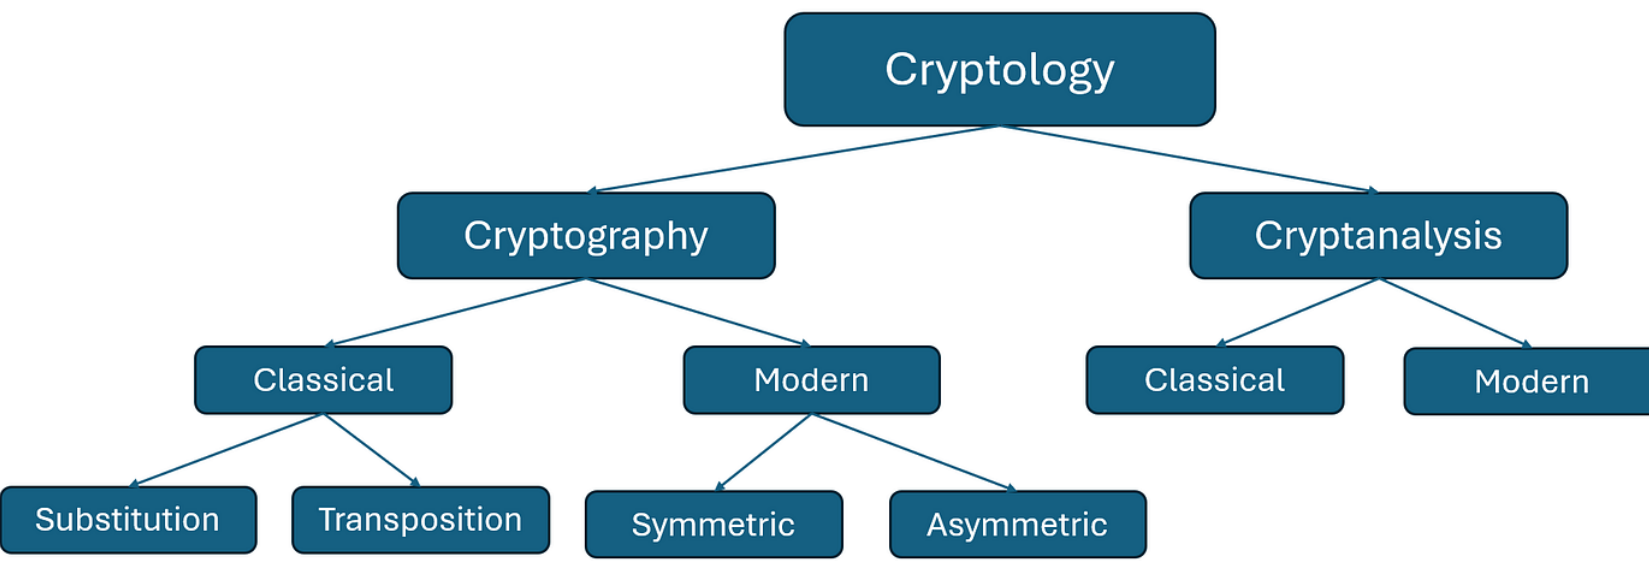
\includegraphics[width=180.39mm,height=154.14mm]{../../images/llm/page_005_img_01.png}%
\end{textblock*}

\end{document}
